\begin{ledgroupsized}[r]{120mm}
\footnotesize
\pstart
\noindent\textbf{\"{U}berlieferung:}
\pend
\end{ledgroupsized}
\begin{ledgroupsized}[r]{114mm}
\footnotesize
\pstart \parindent -6mm
\makebox[6mm][l]{\textit{L}}%
Aufzeichnung: LH XXXVII 5 Bl. 210-211.
1 Bog. 2\textsuperscript{o}.
1 \nicefrac{1}{3} S. auf Bl. 210.
Bl. 211~r\textsuperscript{o} ist leer.
Bl. 211~v\textsuperscript{o} überliefert N. 24. % F/6 = 037,05_211
Ein Wasserzeichen auf Bl. 211.\\%
Cc 2, Nr. 968 B
\pend
\end{ledgroupsized}
%
\vspace*{5mm}
\begin{ledgroup}
\footnotesize
\pstart
\noindent\footnotesize{\textbf{Datierungsgr\"{u}nde}:
Das vorliegende Stück N. 23 % F/5 = 037,05_210
knüpft unmittelbar an die Thematik an,
die in den Stücken N. 19-22 % F/1-4 = 037,05_201, 037,05_204, 037,05_202-203, 037,05_209
in Anlehnung an Galileis\protect\index{Namensregister}{\textso{Galilei} (Galilaeus, Galileus), Galileo 1564-1642}
Ausführungen im zweiten Dialog der \textit{Discorsi e dimostrazioni matematiche} behandelt wird,
nämlich die Bruchfestigkeit von Balken
(siehe für Einzelheiten die Datierungsgründe sowie den Forschungsapparat der letztgenannten Stücke).
Ferner weist der Bogen, der N.~23 % F/5 = 037,05_210
überliefert, das gleiche Wasserzeichen auf wie die Textträger der Stücke N. 19-21. % F/1-3 = 037,05_201, 037,05_204, 037,05_202-203
Demgemäß wird die Datierung von N. 19-22 % F/1-4 = 037,05_201, 037,05_204, 037,05_202-203, 037,05_209
auch für das vorliegende Stück übernommen.}
\pend
\end{ledgroup}
%
\vspace*{8mm}% PR: Rein provisorisch !!!
\normalsize
\count\Afootins=1200
\count\Bfootins=1200
\count\Cfootins=1200
\pstart\noindent
\begin{window}[0,r,\hspace{3mm}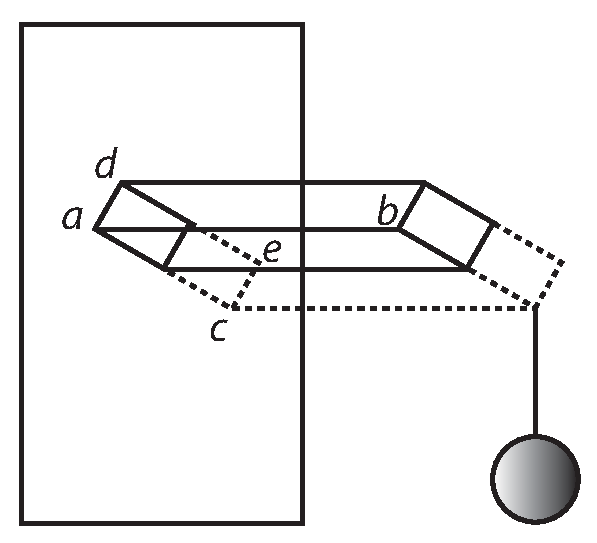
\includegraphics[%trim = -3mm -2mm 0mm 0mm, clip,
width=0.42\textwidth]
{images/lh03705_210r-d1.pdf},\hspace{25mm} {[\textit{Fig. 1}] \vspace{4mm}}]
\noindent
[210~r\textsuperscript{o}] Si trabs\protect\index{Sachverzeichnis}{trabs} ita muro infixa sit, ut axis quidem ejus \edtext{$ab$}{\lemma{\hspace{1.8mm}12\hspace{1.8mm}}\killnumber\Bfootnote{$ab$ \textit{erg. L}}} sit muro\protect\index{Sachverzeichnis}{murus} perpendicularis, \edtext{seu horizonti parallelus,}{\lemma{12f.\hspace{1.8mm}seu}\killnumber\Bfootnote{%
\textit{(1)} horizontalis %
\textit{(2)} horizonti parallelus, \textit{L}}} sed altitudo ejus \edtext{$ac$}{\lemma{13\hspace{1.8mm}}\killnumber\Bfootnote{$ac$ \textit{erg. L}}} non sit horizonti perpendicularis, reddenda est ratio firmitatis\protect\index{Sachverzeichnis}{firmitas}, et augetur {difficultas,\reversemarginpar\marginnote{\scriptsize\hspace{-13mm}15}} \edtext{cum minor}{\lemma{15 \hspace{1.8mm}cum}\killnumber\Bfootnote{\textit{(1)} nulla per \textit{(2)} minor \textit{L}}} est $ad$.
Quaerendum est ante omnia centrum divulsionis.\protect\index{Sachverzeichnis}{centrum divulsionis}
Manifestum est divulsionem non fieri circa $ac$ nec circa $ce$.
Si plane esset jacens foret circa $ac$.
Si plane erectus foret circa $de$.
\newline%
\hspace*{7,5mm}%
{Ajo\reversemarginpar\marginnote{\scriptsize\hspace{-13mm}20}} centrum divulsionis\protect\index{Sachverzeichnis}{centrum divulsionis} esse $c$, axem divulsionis lineam horizonti pariter et Tabulae\protect\index{Sachverzeichnis}{tabula} sustinenti parallelam transeuntem per punctum $c$. Ex hoc jam principio in nostra potestate est, calcu-
\end{window}

%\noindent[210~r\textsuperscript{o}]
%\pend
%\pstart
%\begin{wrapfigure}[13]{l}{0.42\textwidth}
%\vspace{-7mm}\centering
%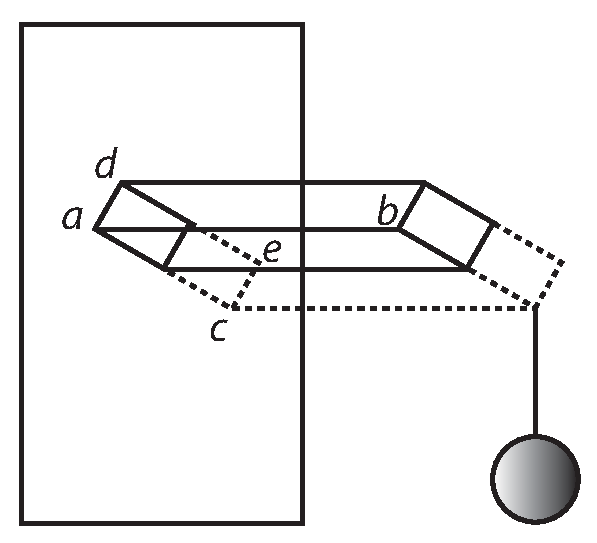
\includegraphics[trim = 1mm -3mm -5mm 0mm, clip, width=0.42\textwidth]{images/lh03705_210r-d1.pdf}\\
%\centering[\textit{Fig. 1}]
%\end{wrapfigure}
%\noindent%
%% [210~r\textsuperscript{o}]
%Si trabs\protect\index{Sachverzeichnis}{trabs} ita muro infixa sit, ut axis quidem ejus \edtext{$ab$}{\lemma{}\Bfootnote{$ab$ \textit{erg. L}}} sit muro\protect\index{Sachverzeichnis}{murus} perpendicularis, \edtext{seu horizonti}{\lemma{seu}\Bfootnote{\textit{(1)} horizontalis \textit{(2)} horizonti \textit{L}}} parallelus, sed altitudo ejus \edtext{$ac$}{\lemma{}\Bfootnote{$ac$ \textit{erg. L}}} non sit horizonti perpendicularis, reddenda est ratio firmitatis\protect\index{Sachverzeichnis}{firmitas}, et augetur difficultas, \edtext{cum minor}{\lemma{cum}\Bfootnote{\textit{(1)} nulla per \textit{(2)} minor \textit{L}}} est $ad$.
%Quaerendum est ante omnia centrum divulsionis.\protect\index{Sachverzeichnis}{centrum divulsionis}
%Manifestum est divulsionem non fieri circa $ac$ nec circa $ce$.
%Si plane esset jacens foret circa $ac$.
%Si plane erectus foret circa $de$.
%\newline%
%\hspace*{7,5mm}%
%Ajo centrum divulsionis\protect\index{Sachverzeichnis}{centrum divulsionis} esse $c$, axem divulsionis lineam horizonti pariter et Tabulae\protect\index{Sachverzeichnis}{tabula} sustinenti parallelam transeuntem per punctum $c$. Ex hoc jam principio in nostra potestate est, calculare
\noindent \setline{24}lare quantitatem, sed generaliter bilanx\protect\index{Sachverzeichnis}{bilanx} mea rem facile determinabit, si eodem \edtext{modo tabula}{\lemma{modo}\Bfootnote{\textit{(1)} res \textit{(2)} tabula \textit{L}}} ex $c$ suspendatur. \pend \pstart Sed quid si neque axis sit horizonti parallelus, neque altitudo perpendicularis. Facilis est calculus ex dictis.
\pend
\newpage% PR: Rein provisorisch !!!
\pstart%
\begin{wrapfigure}[19]{l}{0.47\textwidth}
\vspace{-5mm}\centering
\includegraphics[width=0.47\textwidth]{images/lh03705_210r-d2u3.pdf}\\
\centering\hspace{2.5mm}[\textit{Fig. 2 und 3}]
\end{wrapfigure}%
Data Trabe\protect\index{Sachverzeichnis}{trabs} fulcienda duobus locis, invenire optimum fulciendi modum. Scilicet duo fulcra\protect\index{Sachverzeichnis}{fulcrum} magis appropinquare \edtext{debent extremis quam medio,}{\lemma{debent}\Bfootnote{\textit{(1)} medio, quam extremis \textit{(2)} extremis quam medio, \textit{L}}} quia etsi augeatur praeponderatio tamen in medio ubi ruptura\protect\index{Sachverzeichnis}{ruptura} fieri \edtext{debet}{\lemma{}\Bfootnote{debet \textit{erg. L}}} \edtext{resistentia consideranda}{\lemma{resistentia}\Bfootnote{\textit{(1)} comparanda \textit{(2)} consideranda \textit{L}}} est. Res pendet a longitudine altitudini comparata. Scilicet danda opera est ut $ab$ non praeponderet connexioni $bc$. Nam ut $bd$ praeponderet minor est metus, est enim ei \edtext{superanda dupla}{\lemma{superanda}\Bfootnote{\textit{(1)} sesqui \textit{(2)} dupla \textit{L}}} resistentia\protect\index{Sachverzeichnis}{resistentia} \edtext{alterius in $ab$}{\lemma{alterius}\Bfootnote{\textbar\ in \textit{erg.} \textbar\ $ab$ \textit{L}}} nimirum dimidia resistentia\protect\index{Sachverzeichnis}{resistentia} in $bc$ et dimidia in $d$. Ergo duplo ponderosius debet esse $ab$ quam $cd$. Ergo si longitudo $ab$ sit 1 longitudo $cd$ poterit esse Rq. 2.
\newline% PR: Rein provisorisch !!! 
\hspace*{7,5mm}%
Imo vero alius est calculus nec \edtext{resistentia\protect\index{Sachverzeichnis}{resistentia} vere}{\lemma{resistentia}\Bfootnote{\textit{(1)} fere \textit{(2)} vere \textit{L}}} dupla, ob mirabilem naturam nisus in $d$ accurate excutiendam et \edtext{[considerandam]}{\lemma{}\Bfootnote{considerandum \textit{L \"{a}ndert Hrsg.}}} solutionem ex centro nondum totam absolutam cum absoluta in centro $d$. 
\pend
\pstart%
\begin{wrapfigure}{l}{0.47\textwidth}
\vspace{-5mm}\centering
\includegraphics[width=0.28\textwidth]{images/lh03705_210r-d5.pdf}\\
\centering[\textit{Fig. 4}]
\end{wrapfigure}%
Considerandum de fractura\protect\index{Sachverzeichnis}{fractura ovi} ovi, cur difficulter rumpatur cum in extremis $a. b$ premitur et cur non aeque forte rectangulum. Et considerandum quis in linea pure Elliptica\protect\index{Sachverzeichnis}{linea elliptica} non ovali, quis in parabolica\protect\index{Sachverzeichnis}{linea parabolica} etc. effectus quae sphaerarum, quae fornicum fortitudo. Aliud longe compressio, aliud fractio seu ruptura\protect\index{Sachverzeichnis}{ruptura}.
\pend
\newpage% PR: Rein provisorisch !!! 
\pstart%
\noindent%
% \begin{wrapfigure}{l}{0.50\textwidth}
\centering%
\includegraphics[width=0.47\textwidth]{images/lh03705_210r-d4.pdf}\\
\centering[\textit{Fig. 5}]
% \end{wrapfigure}
\pend
\vspace*{1.5em}% PR: Rein provisorisch !!! 
\pstart%
Ut \setline{1}exacte omnia determinentur, circa rupturam\protect\index{Sachverzeichnis}{ruptura} super duobus fulcris\protect\index{Sachverzeichnis}{fulcrum} fingenda sunt appensa pondera in loco quoque rupturae\protect\index{Sachverzeichnis}{ruptura centralis} \edtext{mediae. In rectis $ab$}{\lemma{mediae.}\Bfootnote{\textit{(1)} Duo hic sunt conatus compositi \textit{(2)} In rectis $ab$ \textit{L}}} vel $aa.b$ potest intelligi punctum $a$ moveri tum circa centrum $d$ tum circa centrum $b.$ punctum $b$ movetur tantum circa centrum $d.$
\pend
\vspace*{1.5em}% PR: Rein provisorisch !!!
\pstart%
\noindent%
%[210~v\textsuperscript{o}]
[\textit{Auf Bl. 210~v\textsuperscript{o}, mittig:}]
\pend
\vspace*{1.0em}% PR: Rein provisorisch !!!
\pstart%
\noindent%
% \begin{wrapfigure}{l}{0.55\textwidth}
\centering%
\includegraphics[width=0.61\textwidth]{images/lh03705_210v-d1.pdf}\\
\centering[\textit{Fig. 6}]
% \end{wrapfigure}
\pend
% \vspace*{1.5em}% PR: Rein provisorisch !!!
\newpage% PR: Rein provisorisch !!!
\pstart%
% \noindent
\begin{wrapfigure}[5]{l}{0.2\textwidth}
\vspace{-5mm}
\includegraphics[trim = 0mm 0mm -5mm 0mm, clip, width=0.2\textwidth]{images/lh03705_210v-d2.pdf}\\
\centering[\textit{Fig. 7}]
\end{wrapfigure}
Ut trabs\protect\index{Sachverzeichnis}{trabs} $abcdef$ rumpatur centraliter seu in $e$
necesse est elidi $eabc$ ac proinde id non gravare in centrali ruptura.\protect\index{Sachverzeichnis}{ruptura centralis}
Porro quantus est conatus in $a$ tantus est in $f$ et aliis omnibus arcus punctis.
Ergo si triangulum $hik$ repraesentet momentum resistentiae\protect\index{Sachverzeichnis}{resistentia} in $af$
et parallelogrammum [\textit{Text bricht ab.}]
\pend
%\vspace*{2.0em}%% PR: Rein provisorisch !!!
%\pstart%
%\noindent%
%\centering%
%\includegraphics[width=0.18\textwidth]{images/lh03705_210v-d2.pdf}\\
%\rule[0pt]{0mm}{6mm} [\textit{Fig. 7}]
%\pend
\count\Afootins=1500
\count\Bfootins=1500
\count\Cfootins=1500